\documentclass{../../PublicResources/DocClass}

    \DocumentTitle{「代码\&数据结构\&算法」学习笔记}
    \DocumentCreatedDate{2020/2/18}

    \LinkBlogPost{}
    \LinkPDFSource{}
    \LinkVideo{}

    \AuthorName{Mr. Kin}
    \AuthorEmail{im.misterkin@gmail.com}
    \AuthorBlog{https://mister-kin.github.io/}

\begin{document}
    \pagenumbering{Roman} % 大写罗马字母样式页码。
    \maketitle
    \addcontentsline{toc}{chapter}{封面}
    \frontmatter
    \phantomsection
\begin{center}
    {\bfseries\sffamily\Large 关于作者}
\end{center}
\addcontentsline{toc}{chapter}{关于作者}

\subsection*{\bfseries \sffamily 关于我}
\begin{wrapfigure}[3]{L}{60pt}
    \vspace*{-20pt}
    \centering
    
\includegraphics{kin-logo}
\end{wrapfigure}
\textbf{Mr. Kin},广东客家仁,程序猿,CG和游戏爱好者,一枚极客。翻译UP主,个人UP主。不定时在B站直播日常:码代码,码博客,翻译,做视频,做教程。 ($\vartheta$$\bullet$\_$\bullet$)$\vartheta$ \hyperlink{follow}{\emph{(点击关注我!)}}

\subsection*{\bfseries \sffamily 开源建设}

\noindent {\bfseries \sffamily 开源软件的中文化翻译}

\begin{itemize}
    \item \href{https://docs.krita.org/zh_CN/}{Krita手册}:2018.8.5 - \href{https://crowdin.com/profile}{2019.4.23}
    \item \href{https://docs.blender.org/manual/zh-hans/latest/}{Blender手册}:2019.7.20 - \href{https://www.blendercn.org/5812.html?tdsourcetag=s_pctim_aiomsg}{2019.9.4} - 至今(\href{https://developer.blender.org/p/Mr_Kin/}{翻译维护})
\end{itemize}

\subsection*{\bfseries \sffamily \hypertarget{contact}{联系方式}}
\vspace*{-1ex}
\noindent {\footnotesize \color{red} \em 注:联系时请注明身份,谢谢!}

\begin{itemize}
    \item QQ:\href{tencent://AddContact/?fromId=45&fromSubId=1&subcmd=all&uin=2312463626&website=www.oicqzone.com}{2312463626}\emph{\color{red}(点击号码加好友)}
    \item 邮箱:2312463626@qq.com ; im.misterkin@gmail.com
\end{itemize}

\subsection*{\bfseries \sffamily \hypertarget{follow}{关注渠道}}
\vspace*{-1ex}
\noindent {\footnotesize \color{red} \em 注:点击文字即可跳转关注!}
\vspace*{-2ex}

\begin{figure}[htbp]
    \centering
    
\includegraphics[scale=0.2]{WechatOfficialAccounts.png}
\end{figure}
\vspace*{-4ex}

\begin{figure}[htbp]
    \centering
    \begin{minipage}[t]{0.2\textwidth}
        \centering
        \caption*{\href{https://mister-kin.github.io}{博客 - Blog}}
        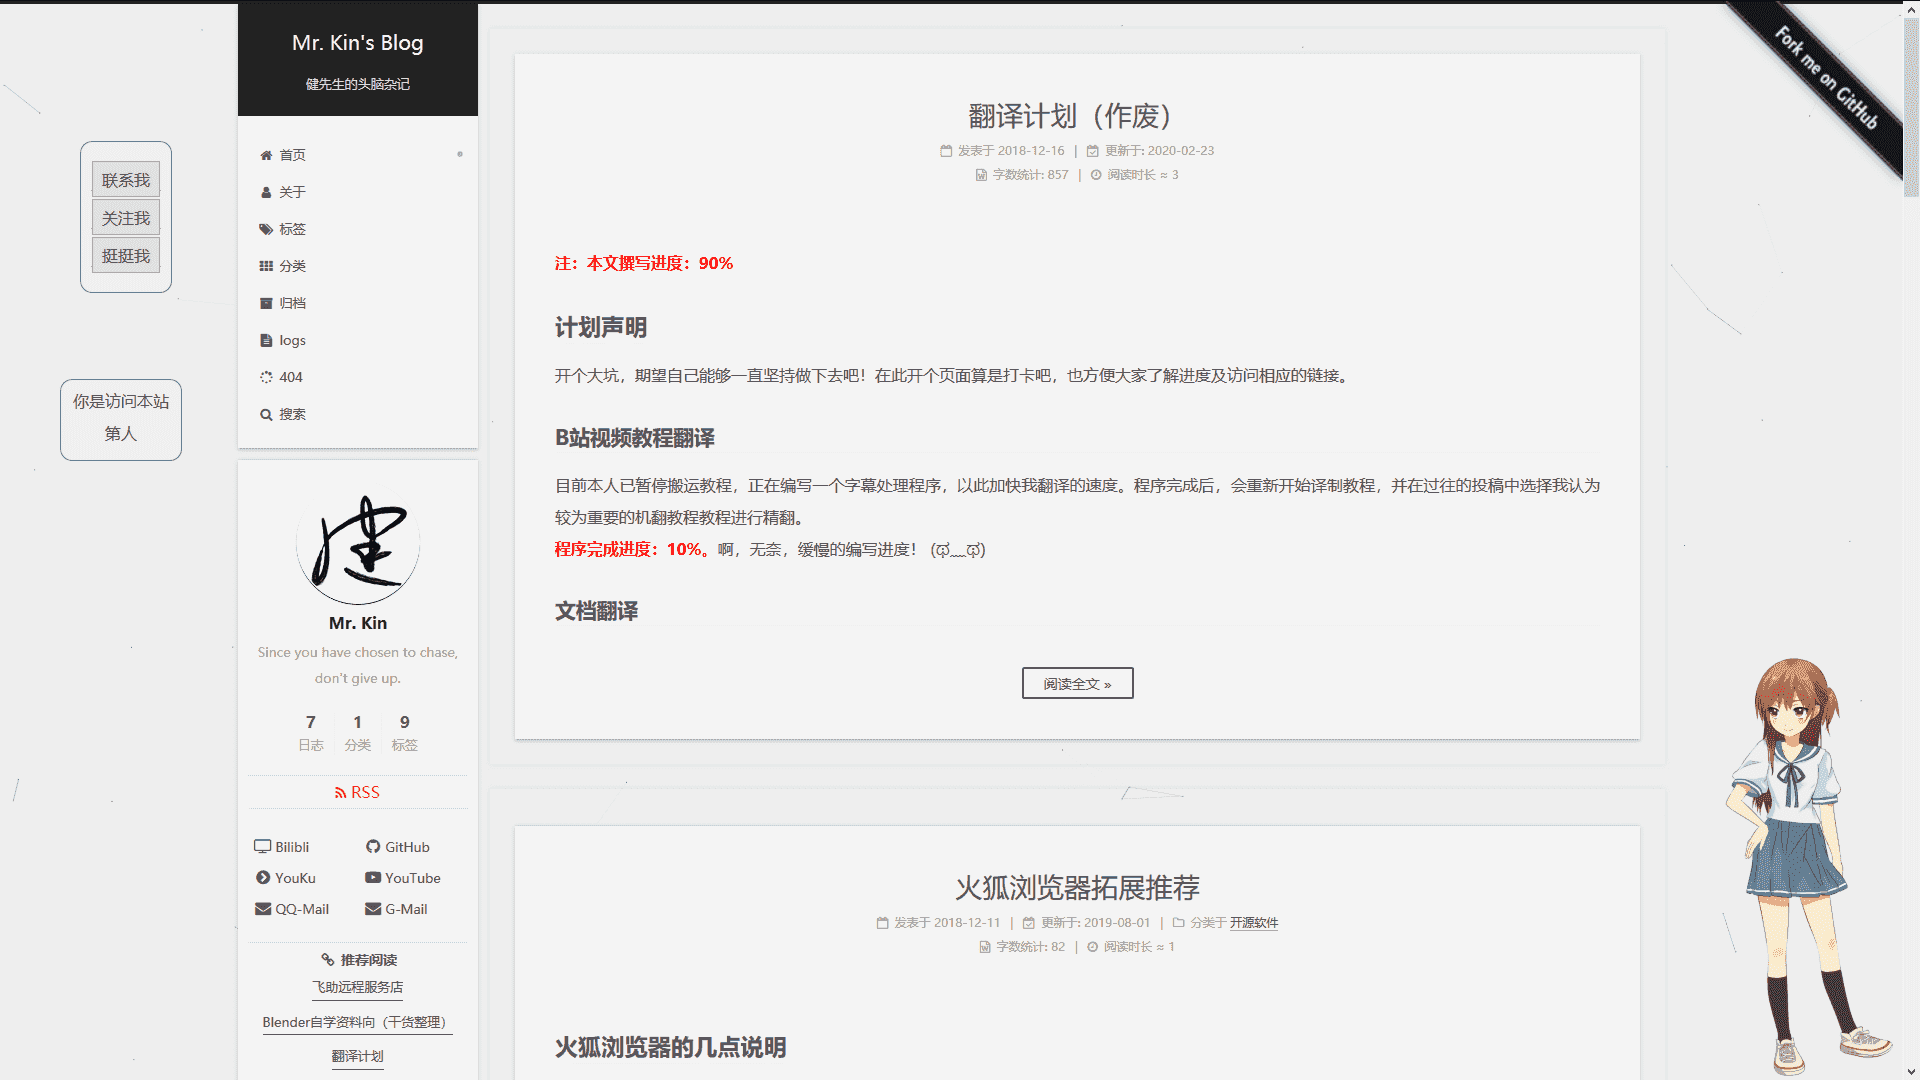
\includegraphics[scale=0.055]{Blog}
    \end{minipage}
    \qquad
    \begin{minipage}[t]{0.2\textwidth}
        \centering
        \caption*{\href{https://github.com/mister-kin}{Github}}
        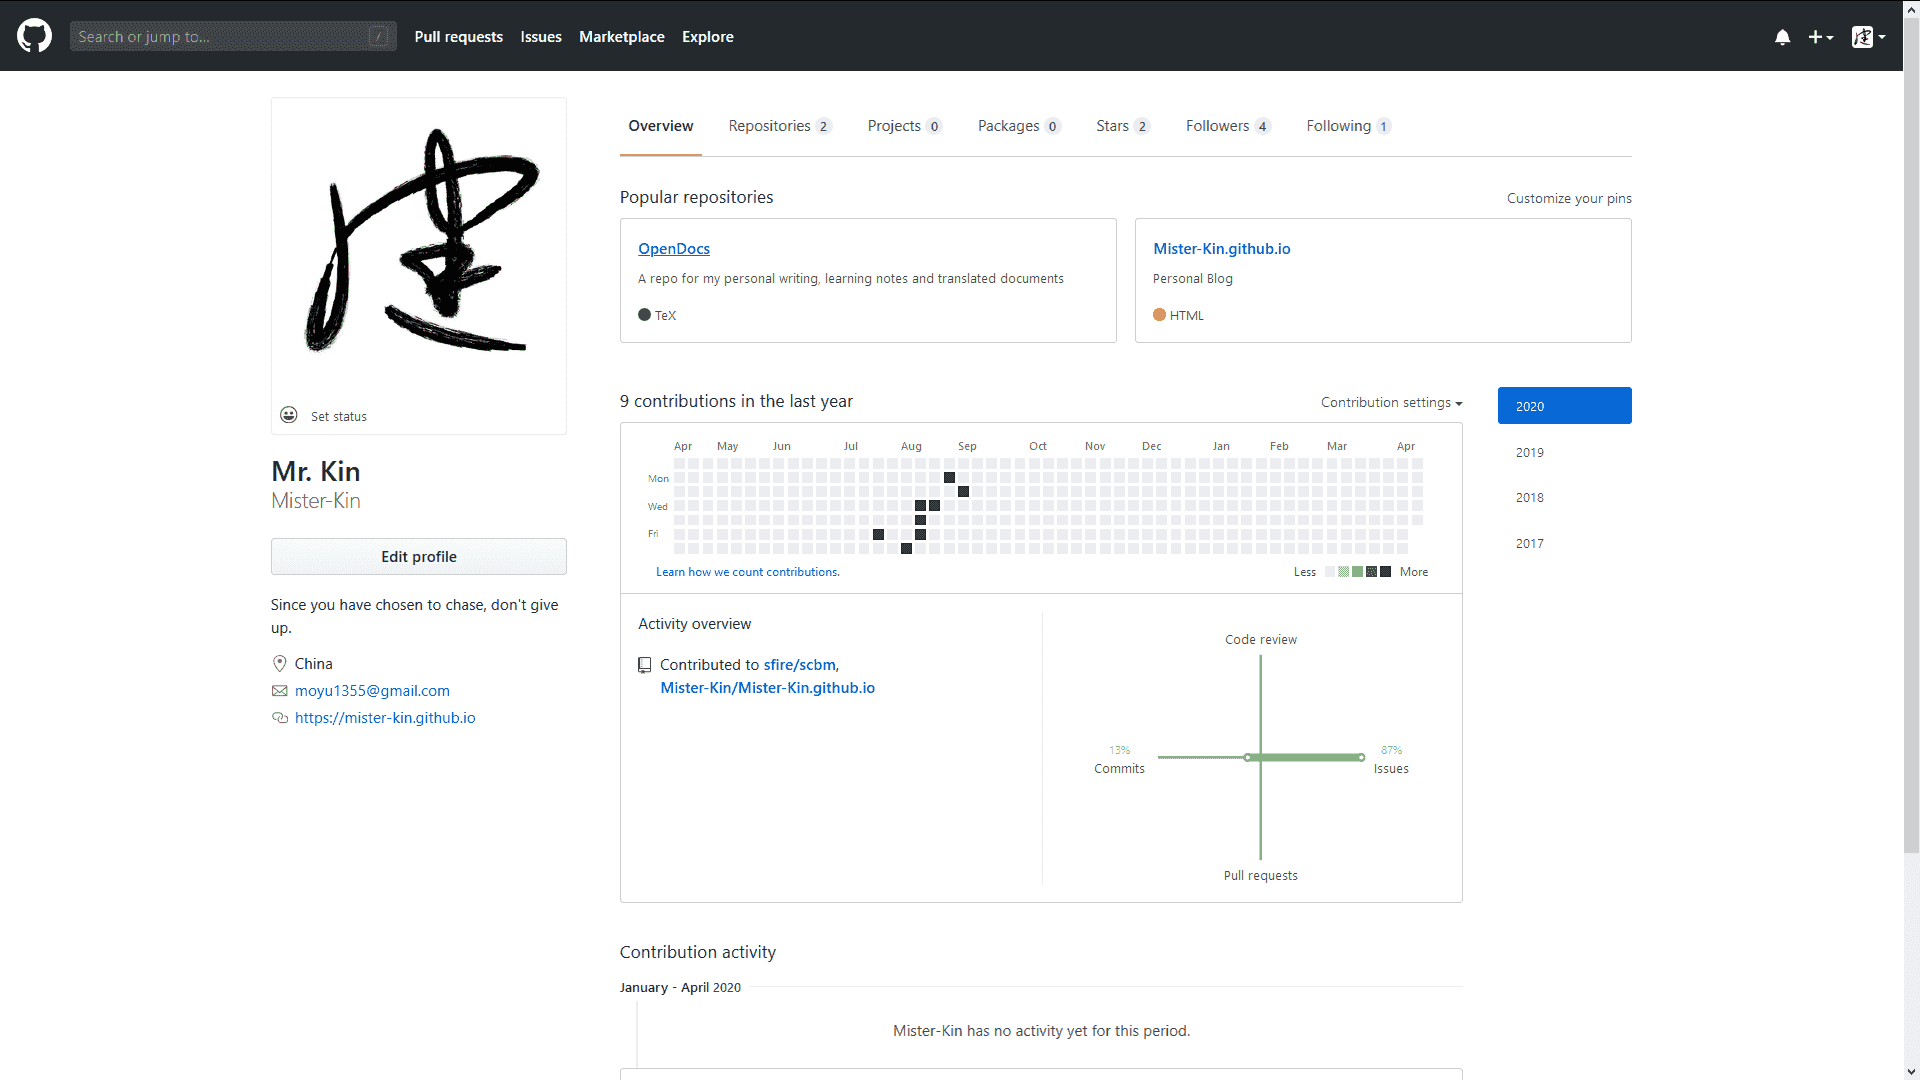
\includegraphics[scale=0.055]{Github}
    \end{minipage}
    \qquad
    \begin{minipage}[t]{0.2\textwidth}
        \centering
        \caption*{\href{https://weibo.com/6270111192/profile?topnav=1&wvr=6&is_all=1}{微博 - Weibo}}
        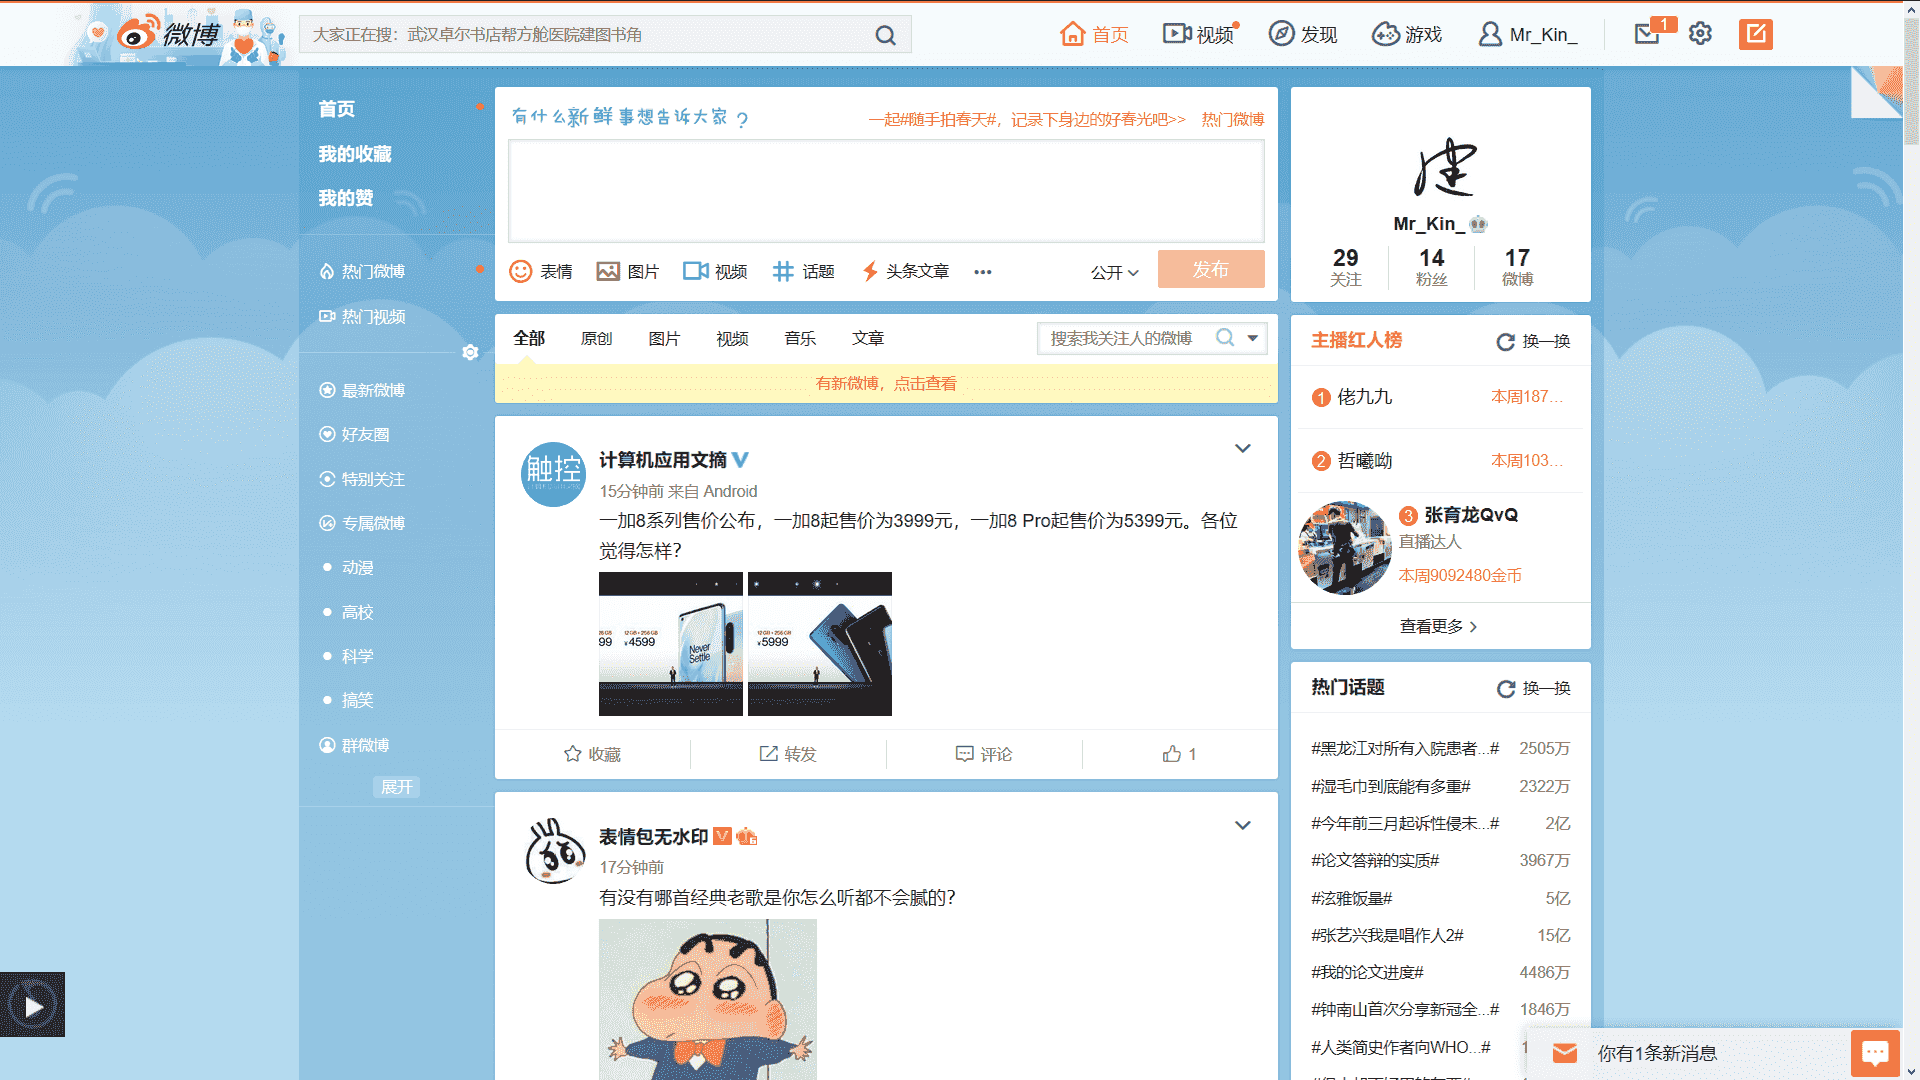
\includegraphics[scale=0.055]{Weibo}
    \end{minipage}
    \qquad
    \begin{minipage}[t]{0.2\textwidth}
        \centering
        \caption*{\href{https://www.zhihu.com/people/drwu-94}{知乎 - Zhihu}}
        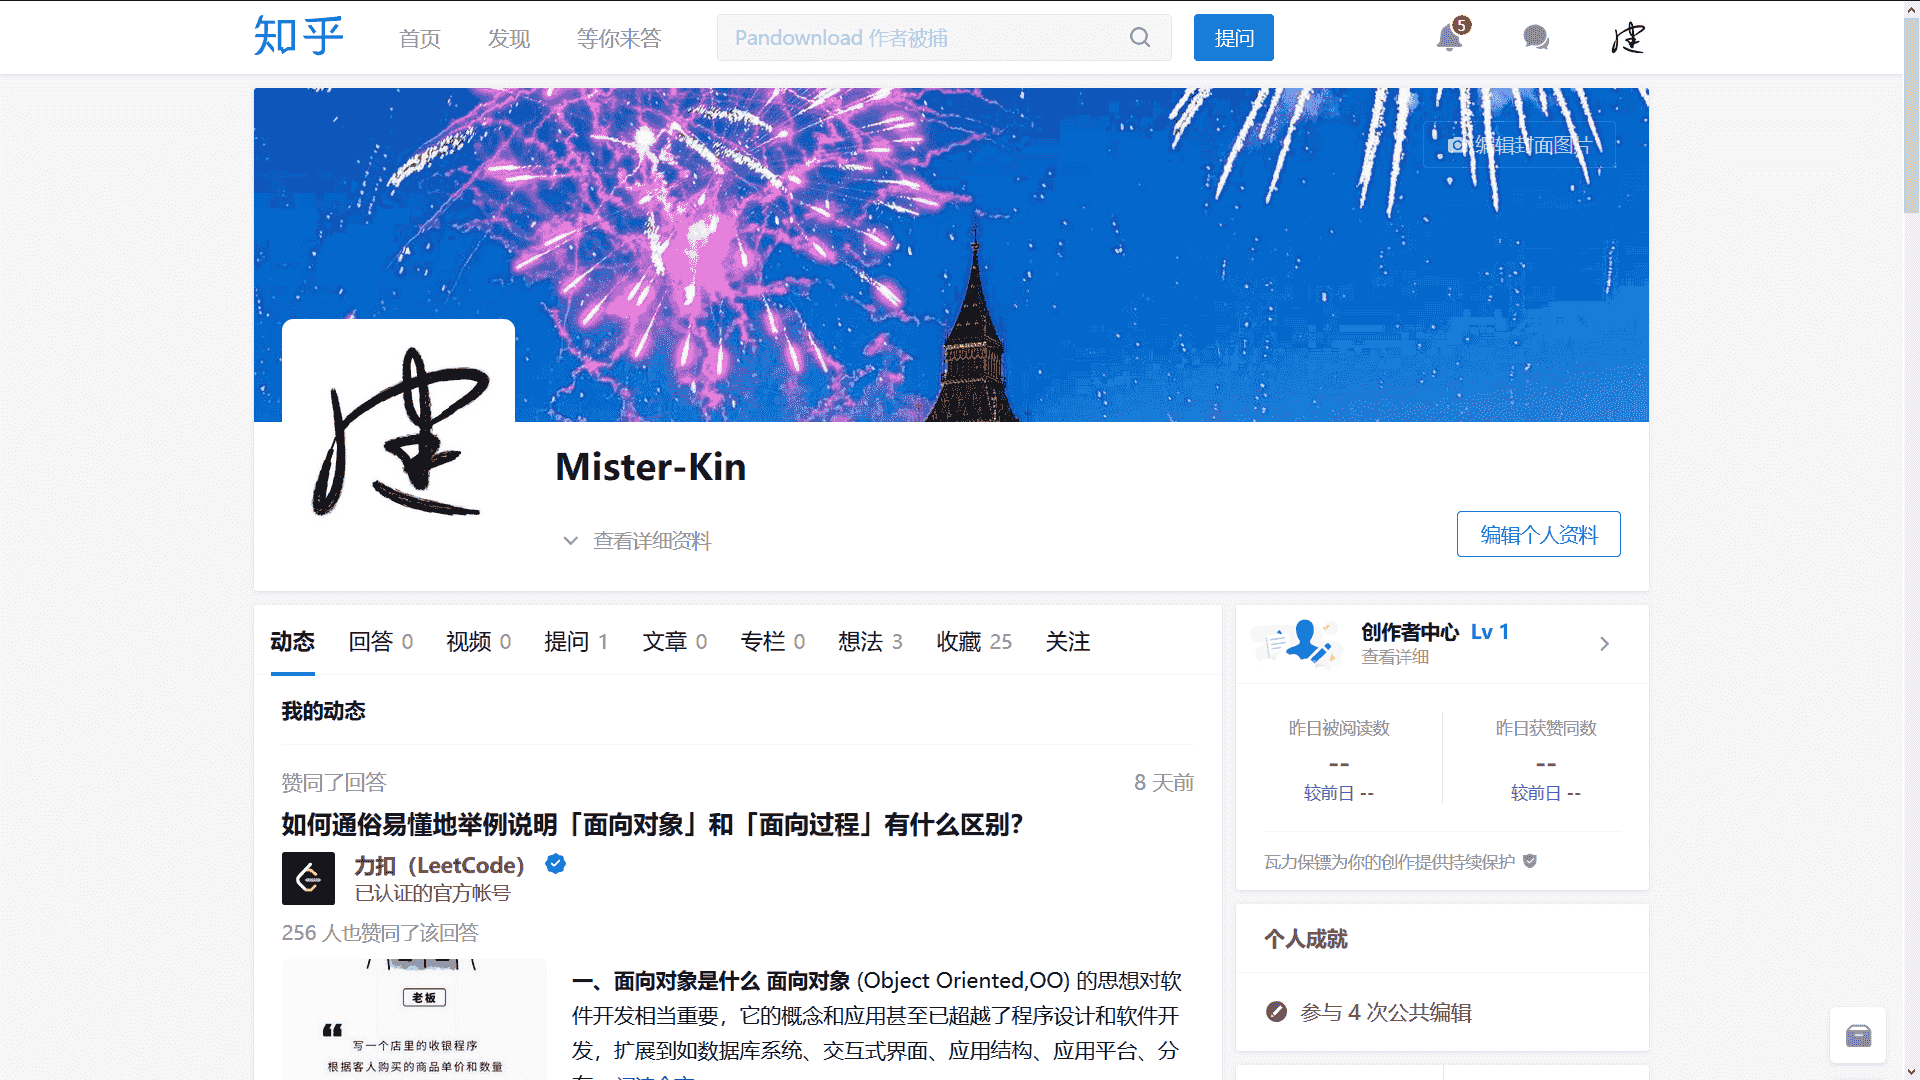
\includegraphics[scale=0.055]{Zhihu}
    \end{minipage}

    \vspace*{3ex}

    \begin{minipage}[t]{0.2\textwidth}
        \centering
        \caption*{\href{http://space.bilibili.com/17025250?}{B站 - Bilibili}}
        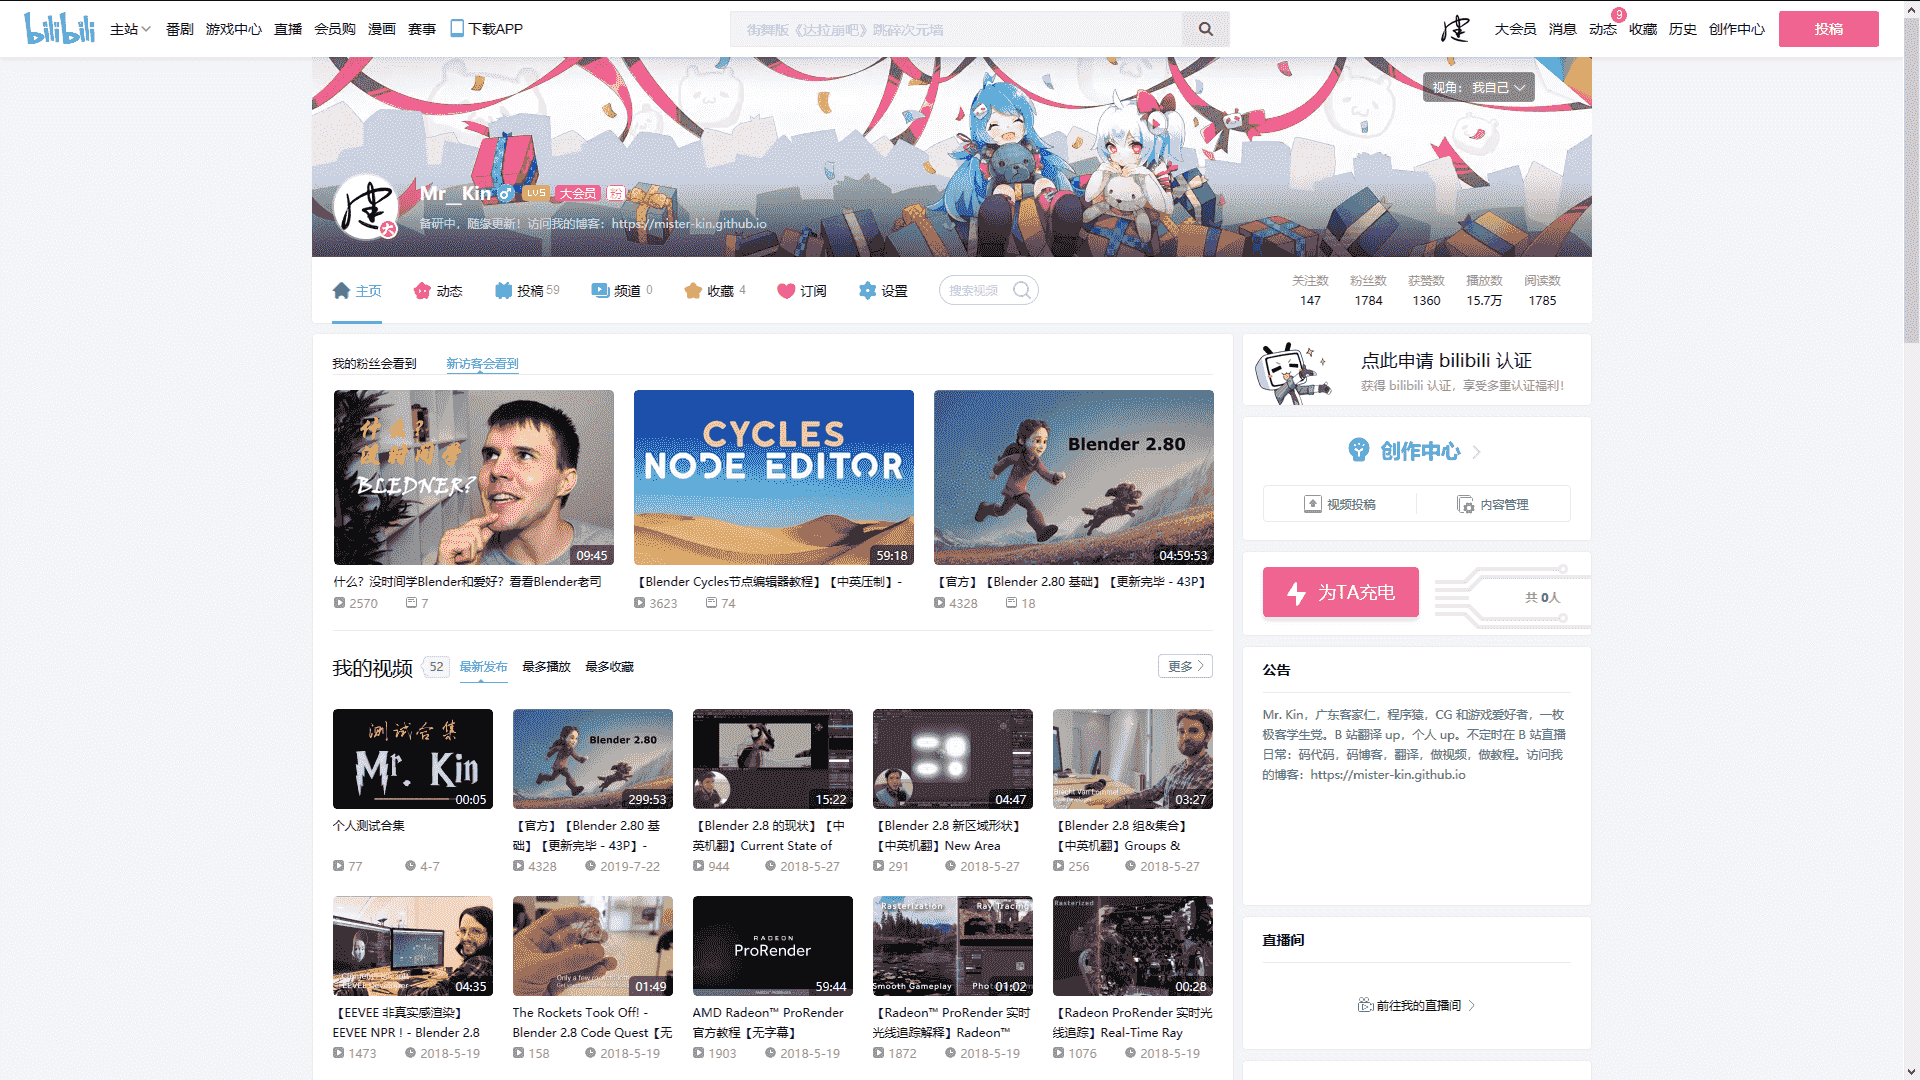
\includegraphics[scale=0.055]{Bilibili}
    \end{minipage}
    \qquad
    \begin{minipage}[t]{0.2\textwidth}
        \centering
        \caption*{\href{http://i.youku.com/i/UNjA3MTk5Mjgw?spm=a2hzp.8253869.0.0}{优酷 - Youku}}
        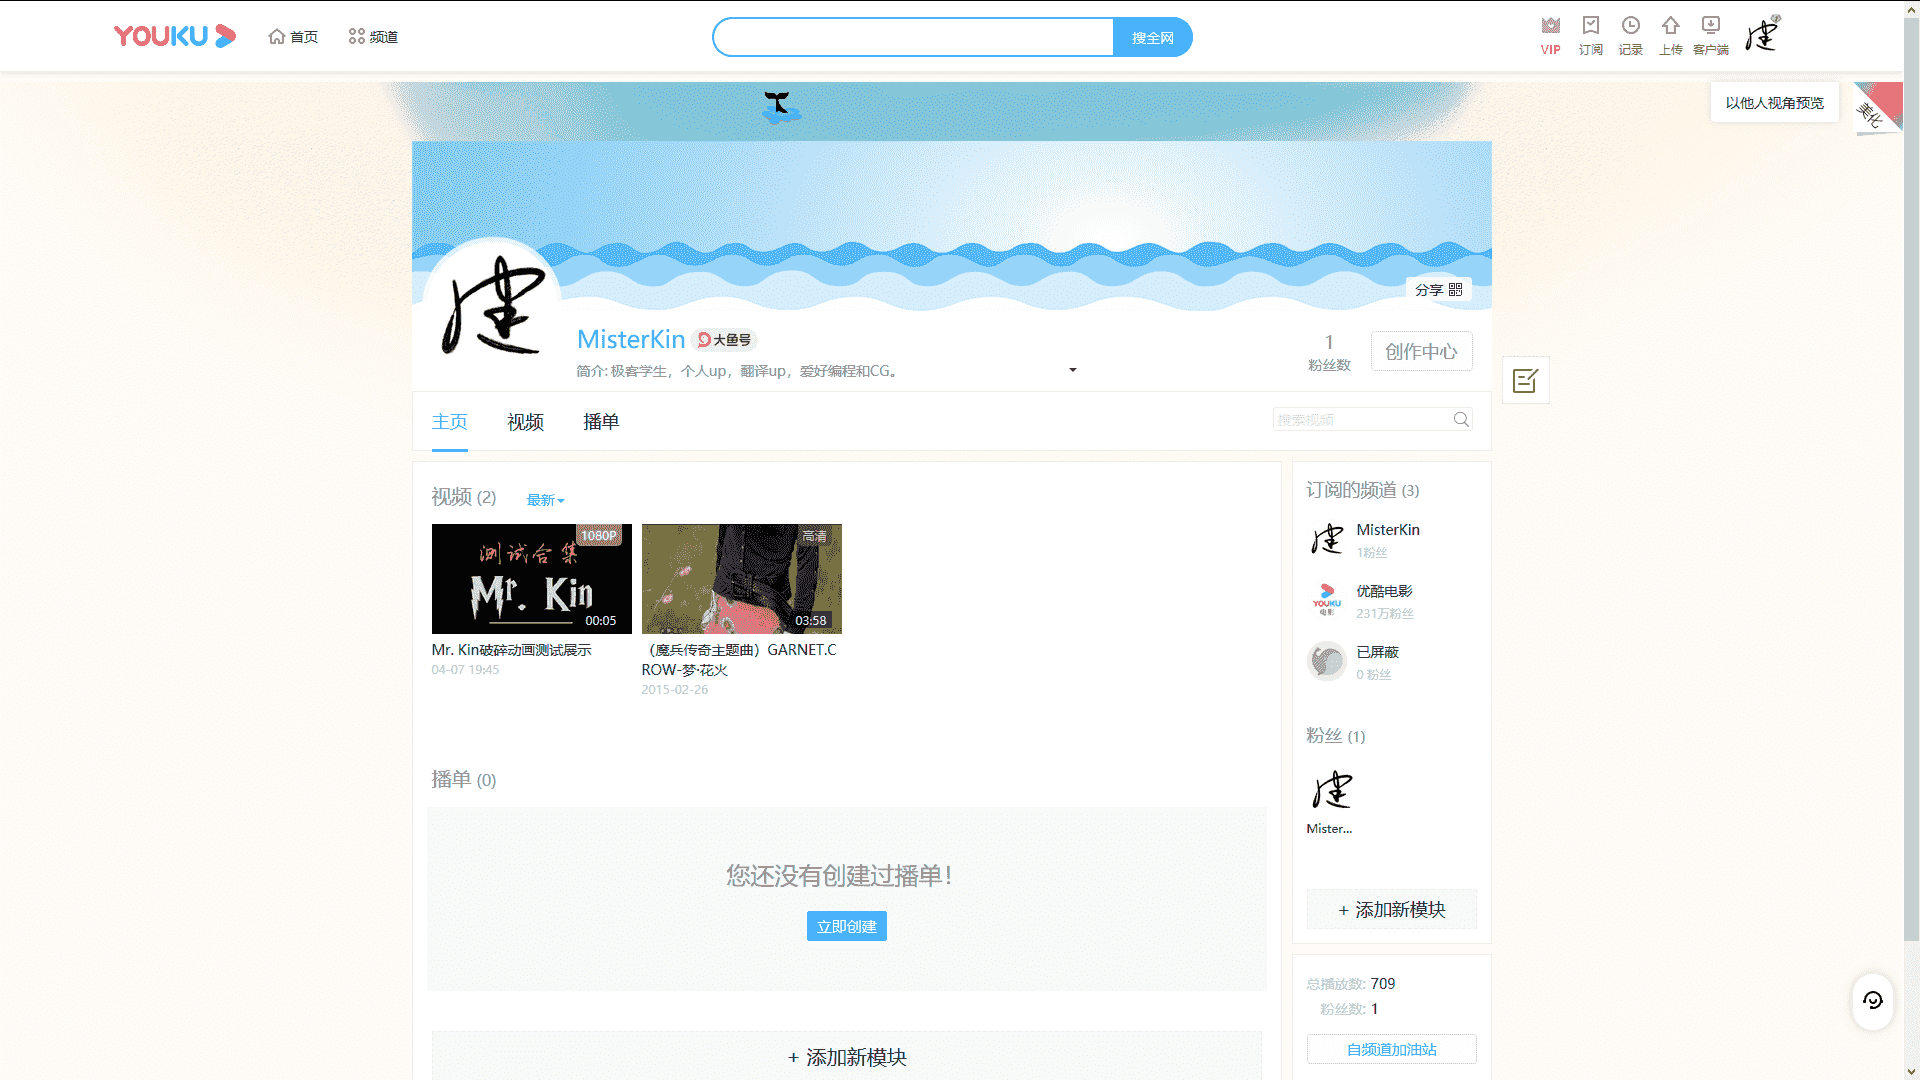
\includegraphics[scale=0.055]{Youku}
    \end{minipage}
    \qquad
    \begin{minipage}[t]{0.2\textwidth}
        \centering
        \caption*{\href{https://www.toutiao.com/c/user/835254071079053/\#mid=1663279303982091}{头条 - Headline}}
        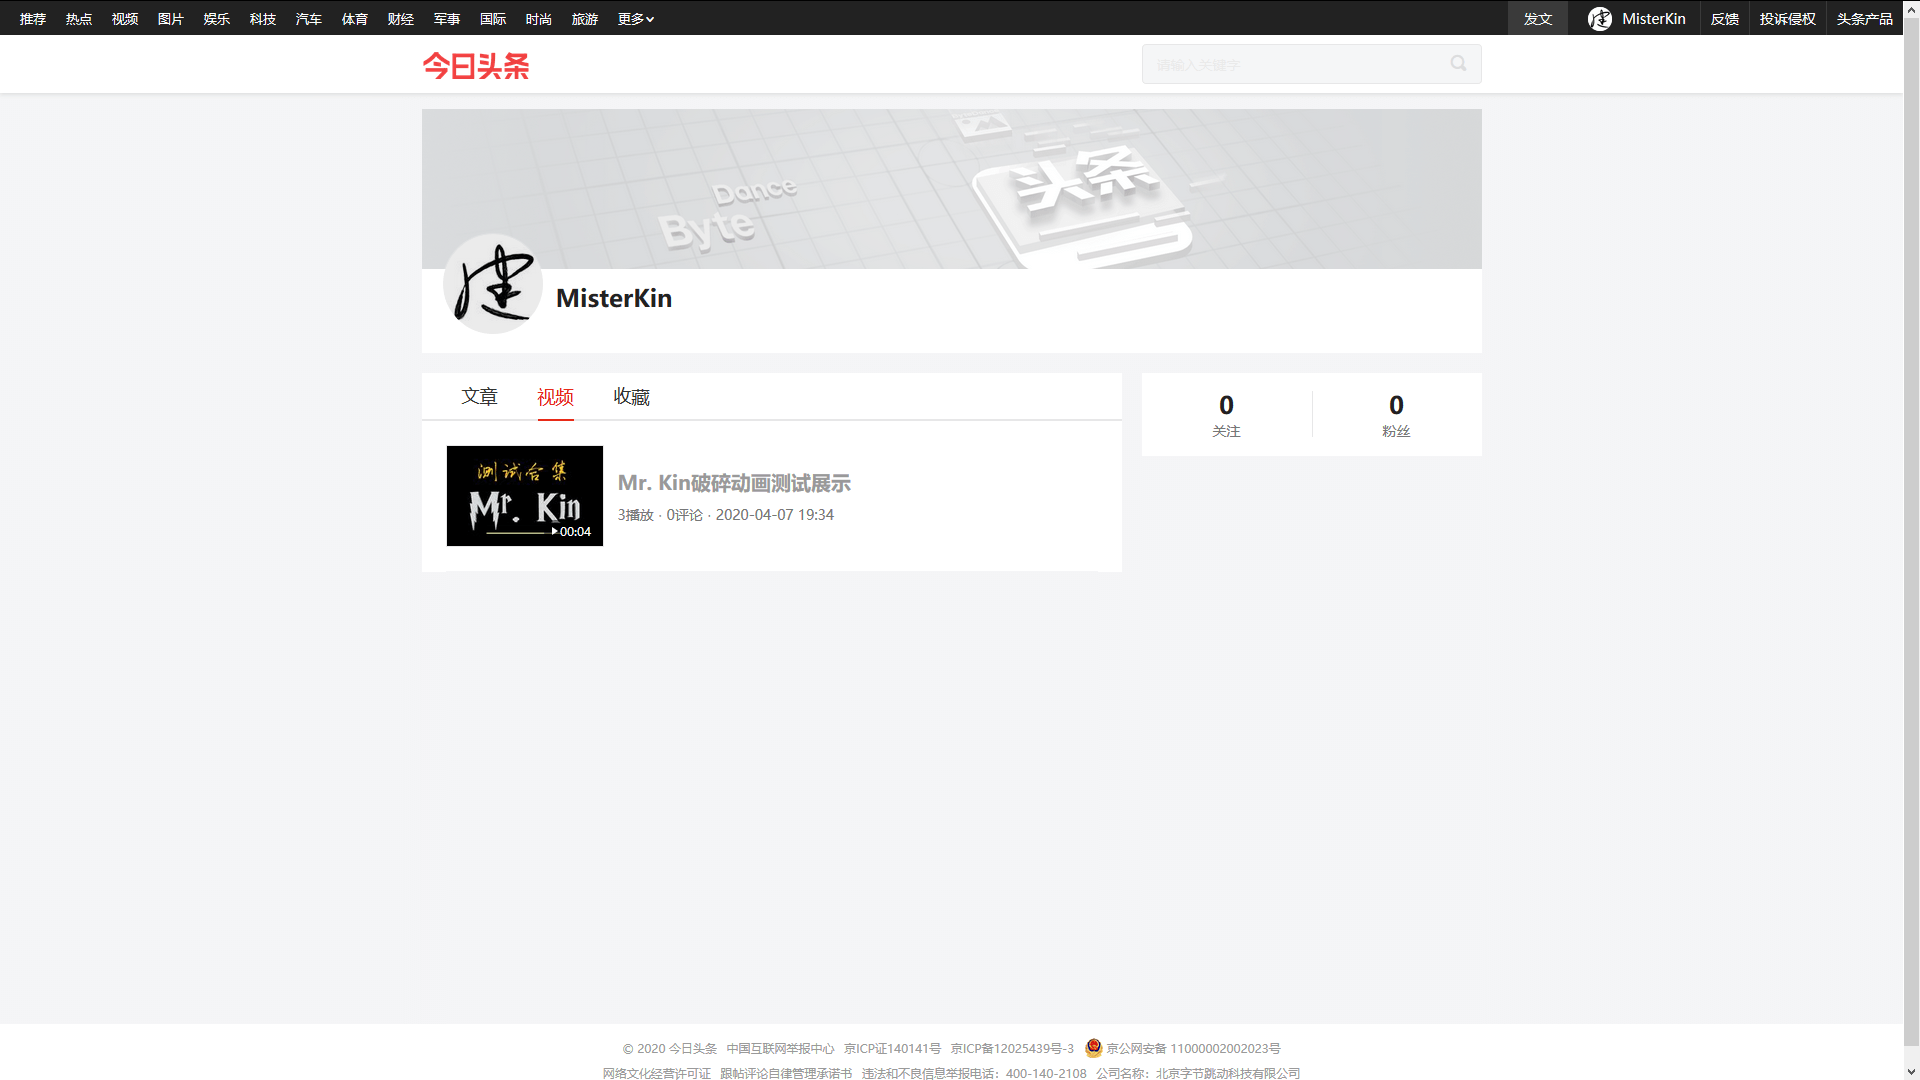
\includegraphics[scale=0.055]{Headline}
    \end{minipage}
    \qquad
    \begin{minipage}[t]{0.2\textwidth}
        \centering
        \caption*{\href{https://www.youtube.com/channel/UCXqjfWLzMlRKxGC8syWj17Q?view_as=public}{油管 - Youtube}}
        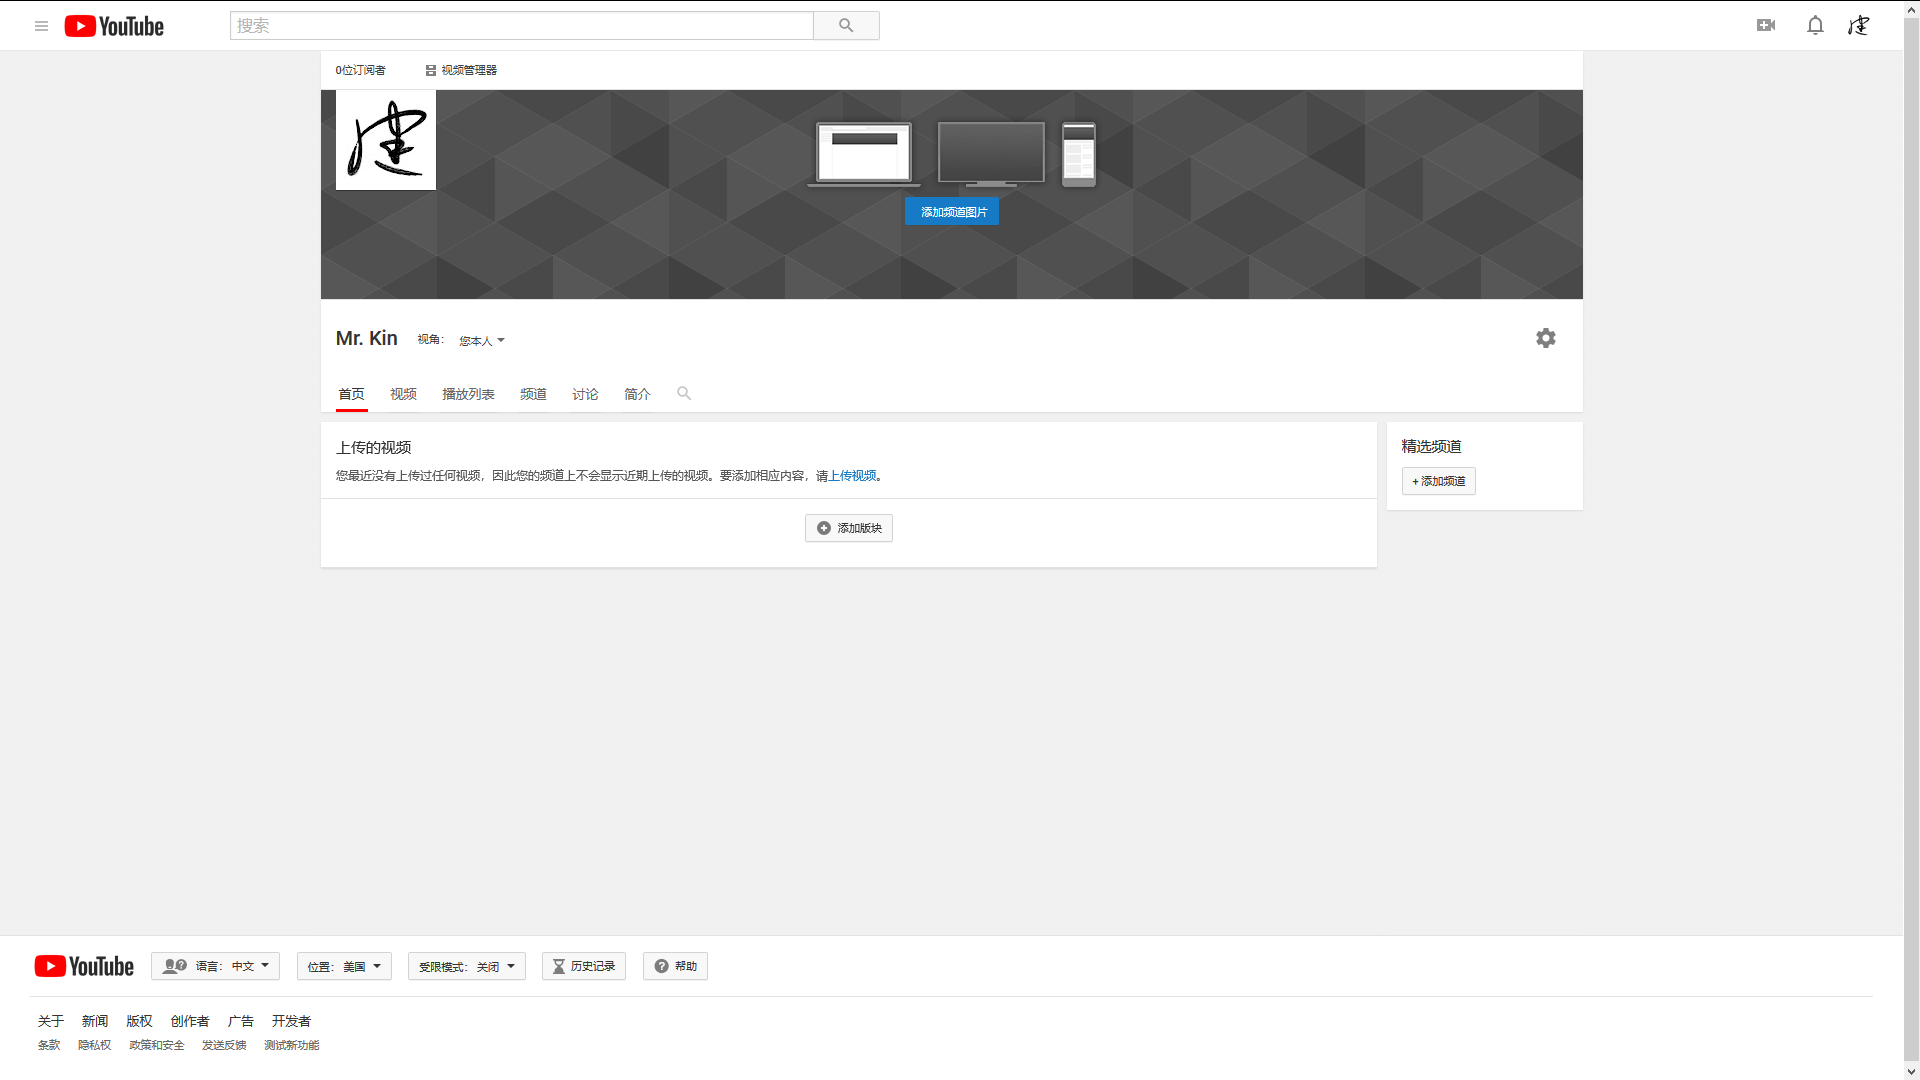
\includegraphics[scale=0.055]{Youtube}
    \end{minipage}
\end{figure}
 % 出于特殊的安全设置,\include 命令无法使用相对路径,因为需要读写权限以给 included file 写 aux 文件,而 \input 命令只需要读权限。
    \clearpage
    \phantomsection
\begin{center}
    {\bfseries\sffamily\Large 版权声明}
\end{center}
\addcontentsline{toc}{chapter}{版权声明}

\noindent 作者:Mr. Kin \\
\DetectToksEmpty\LinkBlogPost
\ifToksEmpty
博文链接:链接暂空\\
\else
博文链接:\href{\the\LinkBlogPost}{跳转博文页}\\
\fi
\DetectToksEmpty\LinkPDFSource
\ifToksEmpty
PDF及LaTex源码链接:链接暂空\\
\else
PDF及LaTex源码链接:\href{\the\LinkPDFSource}{跳转PDF及LaTex源码页}\\
\fi
\DetectToksEmpty\LinkVideo
\ifToksEmpty
\else
相关视频创作链接:\href{\the\LinkVideo}{跳转视频页}\\
\fi
许可协议:本作品的所有内容,除个人设计创作的图像(如logo等)和相关的视频创作及其他特别声明外,均采用\href{https://creativecommons.org/licenses/by-nc-sa/4.0/deed.zh}{知识共享\ 署名-非商业性使用-相同方式共享 4.0 国际许可协议}进行发布。版权 © Mr. Kin,保留所有权利。
\includegraphics[scale=.4]{CC-BY-NC-SA}\\*[1.3ex]
\begin{tabular}{|*{3}{p{0.306\textwidth}|}}
    \hline
    \textsf{\bfseries 允许} & \textsf{\bfseries 限制} & \textsf{\bfseries 条件} \\
    \hline
    \vspace{-8pt}{\color{green}√} 修改 & \vspace{-8pt}{\color{red}×} 商标使用 & \vspace{-8pt}{\color{blue}$\odot$} 保留原署名 \\[-12pt]
    {\color{green}√} 分发 & {\color{red}×} 专利使用 & {\color{blue}$\odot$} 状态变更说明 \\[-12pt]
    {\color{green}√} 个人使用 & {\color{red}×} 商业使用 & {\color{blue}$\odot$} 相同的许可和版权声明 \\
    \hline
\end{tabular}
\\*[1.3ex]
\emph{注:若想对本作品进行转载、引用亦或是进行二次创作时,请详细阅读上述相关协议内容(若不理解,请点击链接跳转阅读)。为保障本人权利,对于违反者,本人将依法予以处理!望周知!——Mr. Kin}

\begin{center}
    {\bfseries\sffamily\Large 勘误声明}
\end{center}

虽本人写作时已尽力保证其内容的正确性,但因个人知识面和经验的局限性以及计算机技术等相关技术日新月异,本作品内容或存在一些错误之处。还望诸君发现错误后能够\hyperlink{contact}{联系我}以更正错误,不胜感激!——Mr. Kin

\begin{center}
    {\bfseries\sffamily\Large 侵权声明}
\end{center}

若本作品采用的第三方内容侵犯了你的版权,请与我\hyperlink{contact}{联系}进行处理,谢谢!——Mr. Kin

\begin{center}
    {\bfseries\sffamily\Large 第三方开源许可声明}
\end{center}

\noindent 本作品使用的第三方开源产品有:
\begin{multicols}{2}
\begin{itemize}
    \item \href{https://github.com/adobe-fonts}{Adobe Fonts}: \href{https://github.com/adobe-fonts/source-serif-pro/blob/release/LICENSE.md}{OFL v1.1}
    \item \href{https://tug.org/texlive/}{Tex Live}: \href{https://tug.org/texlive/copying.html}{TeX Live Licensing}
    \item \href{https://code.visualstudio.com/}{Visual Studio Code}: \href{https://github.com/Microsoft/vscode/blob/master/LICENSE.txt}{MIT}
    \item \href{http://ffmpeg.org/}{FFmpeg}: \href{http://ffmpeg.org/legal.html}{LGPL v2.1 / GPL v2}
    \item \href{https://krita.org/en/}{Krita}: \href{https://docs.krita.org/en/KritaFAQ.html?highlight=license#license-rights-and-the-krita-foundation}{Krita's GPL license}
    \item \href{https://inkscape.org/}{Inkscape}: \href{https://inkscape.org/about/license/}{GPL}
    \item \href{https://www.gimp.org}{GIMP}: \href{https://www.gimp.org/about/COPYING}{GPL}
    \item \href{https://www.blender.org}{Blender}: \href{https://www.blender.org/about/license/}{GPL}
    \item \href{https://www.audacityteam.org/}{Audacity}: \href{https://www.audacityteam.org/about/license/}{GPL v2}
    \item \href{https://handbrake.fr}{Handbrake}: \href{https://github.com/HandBrake/HandBrake/blob/master/LICENSE}{GPL v2}
\end{itemize}
\end{multicols}

\noindent 更多请点击查看\href{https://mister-kin.github.io/about/third-party-declaration/}{第三方声明页}!

    \clearpage
    {\centering \tableofcontents} % 生成目录页。
    \mainmatter

    % 正文
    \chapter{Windows Terminal}

\section{软件自身设置}
快速以管理员身份启动,搜索框内搜索Terminal,ctrl+shift+enter快捷键启动

设置的启动:
\begin{enumerate}
    \item settings.json:下拉菜单>设置
    \item defaults.json:alt键按住+下拉菜单>设置
\end{enumerate}

\begin{lstlisting}[language={bash},title={\textsf{Ternimal的设置:颜色方案和字体大小}}]
    "profiles":
    {
        "defaults":
        {
            // Put settings here that you want to apply to all profiles.
            "colorScheme": "One Half Light",
            "fontSize": 15,
        },
    }
\end{lstlisting}

\section{CMD\&PS}

\chapter{Markdown}

链接中添加空格的方法
使用\&\#32;或者-替代空格

代码块
行内代码:`code` ,反引号`为~键
多行代码:
```language
code
```

\chapter{Python}

\section{PIP工具}
\paragraph{PIP源设定} pip config set global.index-url https://pypi.tuna.tsinghua.edu.cn/simple

\paragraph{Win端PIP缓存路径} \%LocalAppData\%>pip>Cache

临时使用

pip install -i https://pypi.tuna.tsinghua.edu.cn/simple some-package

注意,simple 不能少, 是 https 而不是 http
设为默认

升级 pip 到最新的版本 (>=10.0.0) 后进行配置:

pip install pip -U
pip config set global.index-url https://pypi.tuna.tsinghua.edu.cn/simple

如果您到 pip 默认源的网络连接较差,临时使用本镜像站来升级 pip:

pip install -i https://pypi.tuna.tsinghua.edu.cn/simple pip -U

\chapter{Git}

\section{常规命令行操作}
相当于fetch后merge
git pull origin master

release发布二进制
hub release create -a ../learngit/README.md -m "release my first program" v1.0.1

git clone http链接(可以不包含git后缀)

\chapter{Hexo+Github Pages搭建个人博客}

\section{环境配置}
\subsection{安装NodeJS和Yarn}
注意nodejs不要安装默认附带的npm包管理工具。其他都是一路默认即可,包括yarn。

若想使用npm来管理包,请查看yarn和npm相关对应的命令。
\begin{lstlisting}[language={bash},title={yarn和npm对应命令}]
    yarn add # npm install
    yarn add [package] # npm install [package] --save
    yarn global add [package] # npm install [package] --global
\end{lstlisting}

\noindent {\footnotesize \emph{注 :Node版本选择v12,避免Stylus for Node v14 'Accessing non-existent property' errors。}}

\subsection{Yarn源设定}
\begin{lstlisting}[language={bash},title={\textsf{Yarn源设定命令}}]
    yarn config get registry  // 查看yarn当前镜像源
    yarn config set registry https://registry.npm.taobao.org/  // 设置yarn镜像源为淘宝镜像
\end{lstlisting}

\subsection{安装hexo}
在想要安装hexo的位置建立文件夹「hexo」,右键该文件夹,选择Git Bash。然后执行下面命令(推荐全局安装)。

\noindent {\footnotesize \emph{注:yarn add(hexo init之后)该条命令为可选,因为hexo init之后一般都会自动安装相关依赖。若没有自动安装时,则需要执行该条命令以手动安装依赖。}}

\begin{lstlisting}[language={bash},title={全局安装hexo}]
    yarn global add hexo-cli # 全局安装hexo-cli脚手架
    hexo init # 初始化hexo,克隆hexo-starter和默认landscape主题仓库
    hexo s # hexo server,启用本地服务器,见:http://localhost:4000/
\end{lstlisting}

\begin{lstlisting}[language={bash},title={本地安装hexo}]
    yarn add hexo-cli
    node_modules/.bin/hexo.cmd init blog # init需要空文件夹,所以另外用文件夹「blog」来初始化hexo
    cd blog
    yarn add
    node_modules/.bin/hexo.cmd s
\end{lstlisting}

\subsection{清除yarn已安装的包}
\begin{lstlisting}[language={bash},title={命令查看yarn相关路径}]
    yarn global dir # 全局安装路径
    yarn cache dir # 缓存路径,yarn缓存不会自动删除,省去重复下载
    yarn cache clean # 清理缓存路径
\end{lstlisting}

\section{Config配置}

\begin{intro}
    注意:以下代码中,cd hexo含义均代表:命令执行路径为站点的根目录,即为hexo init命令初始化的路径。以hexo为开头的路径均为:站点根目录/theme/next。「新增相关代码」若无提到位置,则任意位置都可以。
\end{intro}

\subsection{站点Config}
\subsubsection{本地实时预览 - browsersync}
\begin{lstlisting}[language={bash},title={安装插件hexo-browsersync}]
    cd hexo
    yarn add hexo-browsersync
\end{lstlisting}

\subsubsection{网站设置}
\noindent {\footnotesize \emph{注:language根据主题设置,注意新版Next主题已经没有zh-Hans语言配置文件,设置中文简体请用zh-CN参数。}}
\begin{lstlisting}[language={PHP},title={搜索站点Config.yml相关代码并修改}]
    # Site
    title: Mr. Kin's Blog
    subtitle: 健先生的博客
    description: Since you have chosen to chase, don't give up.
    author: Mr. Kin
    language: zh-CN
    timezone: Asia/Shanghai
\end{lstlisting}

\subsubsection{网址设置}
\begin{lstlisting}[language={PHP},title={搜索站点Config.yml相关代码并修改}]
    # URL
    url: https://mister-kin.github.io/
    permalink: :title/ # 仅使用title以优化seo
\end{lstlisting}

\subsubsection{使用第三方主题:Next}
\noindent {\footnotesize \emph{注:新版Next主题主仓库已从 iissnan 名下迁移至 theme-next 组织。}}

\begin{lstlisting}[language={bash},title={下载安装Next主题}]
    cd hexo
    git clone https://github.com/theme-next/hexo-theme-next themes/next
\end{lstlisting}

\begin{lstlisting}[language={PHP},title={搜索站点Config.yml相关代码并修改}]
    # Extensions
    theme: next
\end{lstlisting}

\subsubsection{Github Pages部署配置}
\begin{lstlisting}[language={PHP},title={搜索站点Config.yml相关代码并修改}]
    # Deployment
    deploy:
        type: git
        repo: git@github.com:mister-kin/mister-kin.github.io.git
        branch: master
\end{lstlisting}

\subsection{主题Config}
\subsubsection{选择方案「Scheme」}
\begin{lstlisting}[language={PHP},title={搜索主题Config.yml相关代码并修改}]
    # Schemes
    #scheme: Muse # 注释掉不使用的默认方案
    scheme: Gemini
\end{lstlisting}

\subsubsection{设置「语言」「作者昵称」「站点描述」}
见

\subsubsection{设置「菜单」}
\noindent {\footnotesize \emph{注:现阶段新版Next支持Font Awesome 5.13.0,而5.1.4旧版Next版本只支持Font Awesome 4.7.0}}
\begin{lstlisting}[language={PHP},title={搜索主题Config.yml相关代码并修改}]
    # Menu Settings
    menu:
        home: / || fa fa-home
        about: /about/ || fa fa-user
        tags: /tags/ || fa fa-tags
        logs: /logs || fa fa-file-alt
        commonweal: /404/ || fa fa-spinner
\end{lstlisting}
\begin{lstlisting}[language={PHP},title={搜索next/languages/zh-CN.yml相关代码并修改}]
    menu:
        logs: 日志
        commonweal: '404'
\end{lstlisting}

\subsubsection{设置「头像」}
\noindent {\bfseries \sffamily 加载头像}
在next/source/uploads/路径下新建文件夹「uploads」,并将头像放置于内。
\begin{lstlisting}[language={PHP},title={搜索主题Config相关代码并修改}]
    avatar: /uploads/avatar.webp
\end{lstlisting}
\noindent {\bfseries \sffamily 圆形化头像并旋转}
\begin{lstlisting}[language={PHP},title={next/source/css/main.styl底部新增相关代码}]
    // Customized Contents
    // 导入_custom/custom.styl
    @import "_custom/custom";
\end{lstlisting}

在next/source/css路径下新建文件夹「\_custom」,并新建custom.styl放置于内。
\begin{lstlisting}[language={PHP},title={next/source/css/\_custom/custom.styl新增相关代码}]
    // Customized Contents
    // 圆形化头像并旋转
    @import "../../uploads/css/avatar-round-rotate.styl"
\end{lstlisting}

在next/source/uploads/路径下新建文件夹「css」,并新建avatar-round-rotate.styl放置于内。
\begin{lstlisting}[language={PHP},title={next/source/uploads/avatar-round-rotate.styl新增相关代码}]
    // 配置文件为\themes\next\source\css\_custom\custom.styl。
    // 圆形化头像并旋转

    // 圆形化头像
    if (hexo-config('avatar_custom.round')) {
        .site-author-image {
        border-radius: 50%; // 大于50%效果都一样
        box-shadow: inset 0 -1px 0 #000000;
        }
    }

    // 鼠标经过头像旋转360度
    if (hexo-config('avatar_custom.rotate')) {
        .site-author-image {
        transition: transform 2s ease-out;
        }
        .site-author-image:hover {
        transform: rotateZ(360deg);
        }
    }
\end{lstlisting}

\subsubsection{设置RSS}
\begin{lstlisting}[language={bash},title={安装插件hexo-generator-feed}]
    cd hexo
    yarn add hexo-generator-feed
\end{lstlisting}

\subsubsection{设置代码高亮}
\begin{lstlisting}[language={PHP},title={搜索主题Config相关代码并修改}]
    codeblock:
        highlight_theme: night
        copy_button:
        enable: true
\end{lstlisting}

\subsubsection{设置社交链接}
\begin{lstlisting}[language={PHP},title={搜索主题Config相关代码并修改}]
    # Social links
    social:
\end{lstlisting}


\subsubsection{添加本地搜索 - Local Search}
\begin{lstlisting}[language={bash},title={安装插件hexo-generator-searchdb}]
    cd hexo
    yarn add hexo-generator-searchdb
\end{lstlisting}
\begin{lstlisting}[language={PHP},title={站点Config新增相关代码}]
    search:
        path: search.xml
        field: post
        format: html
        limit: 10000
\end{lstlisting}
\begin{lstlisting}[language={PHP},title={搜索主题Config相关代码并修改}]
    # Local search
    local_search:
        enable: true
\end{lstlisting}

去除推荐阅读(友链),开启fancybox,rss已经是放置于每篇文章背后


    \input{DataStructures/DataStructures}
    \input{Algorithms/Algorithms}

    \nocite{*} % 不使用 cite 也能生成参考文献。
    \printbibliography % 生成参考文献排版。
    \addcontentsline{toc}{chapter}{参考文献} % 添加参考文献进目录。

    \appendix
    % 附录

\end{document}
